\section{MaxPartitions algorithm}%
\label{sec:maxParts}

The idea of the \texttt{MaxPartitions} algorithm is to maximize the size of the
state space partitions, so that the overall number of partitions used to
represent the strategy is minimized. As previously described, the partitioning
that happens during training in UPPAAL Stratego creates a lot of redundant
splits in the state space and this is amplified when we convert the Q-trees to a
unified decision tree.

As an example, take a look at the example strategy in
Figure~\ref{fig:complexExample}. On the left, is the decision tree
representation and on the right is a 2D visualization of the partitioning of the
state space. It is easy to see, that this perfectly valid decision tree entails
a state space partitioning with several redundant partitions, where areas of the
same color (meaning they suggests the same optimal action) are split in two.
Since each confined area, ie.\ partition, is represented in our decision tree as
a leaf node, the fewer partitions we have the smaller a tree we need to
represent it.

\begin{figure}[ht]
    \begin{subfigure}[b]{.5\textwidth}
        \centering
        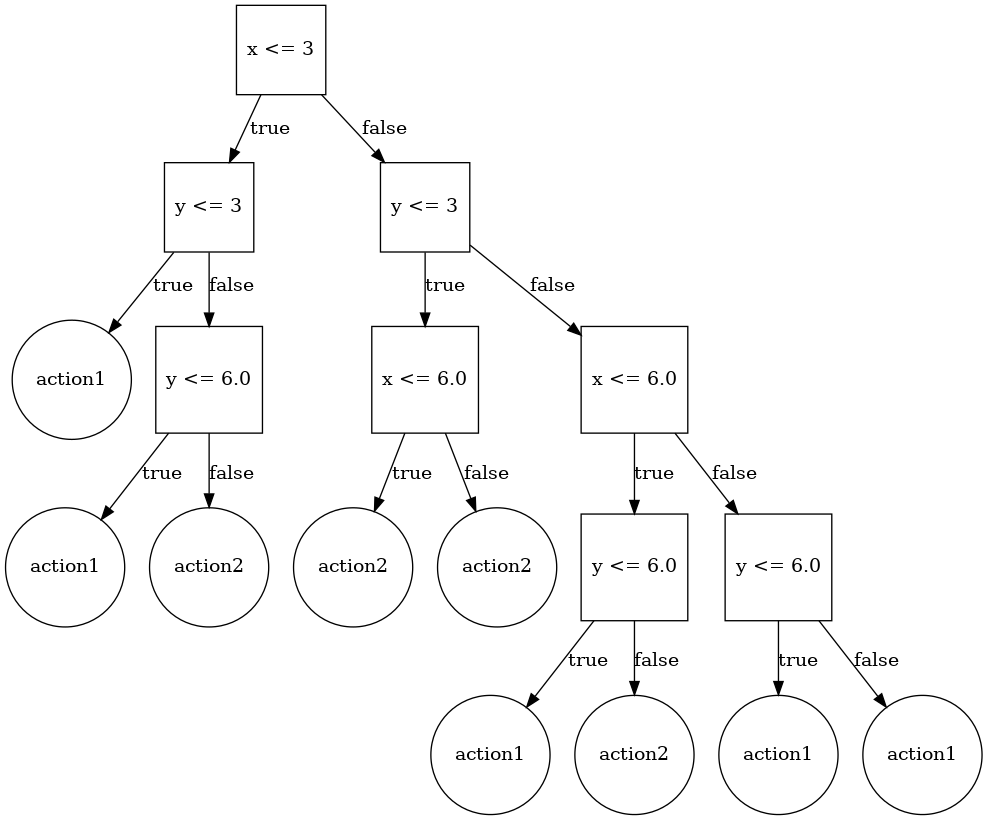
\includegraphics[width=\textwidth]{complexExampleTree}
        \subcaption{%
            % Tree representation of strategy with 2 state dimensions and 3
            % actions
        }\label{fig:complexExampleTree}
    \end{subfigure}
    \begin{subfigure}[b]{.5\textwidth}
        \centering
        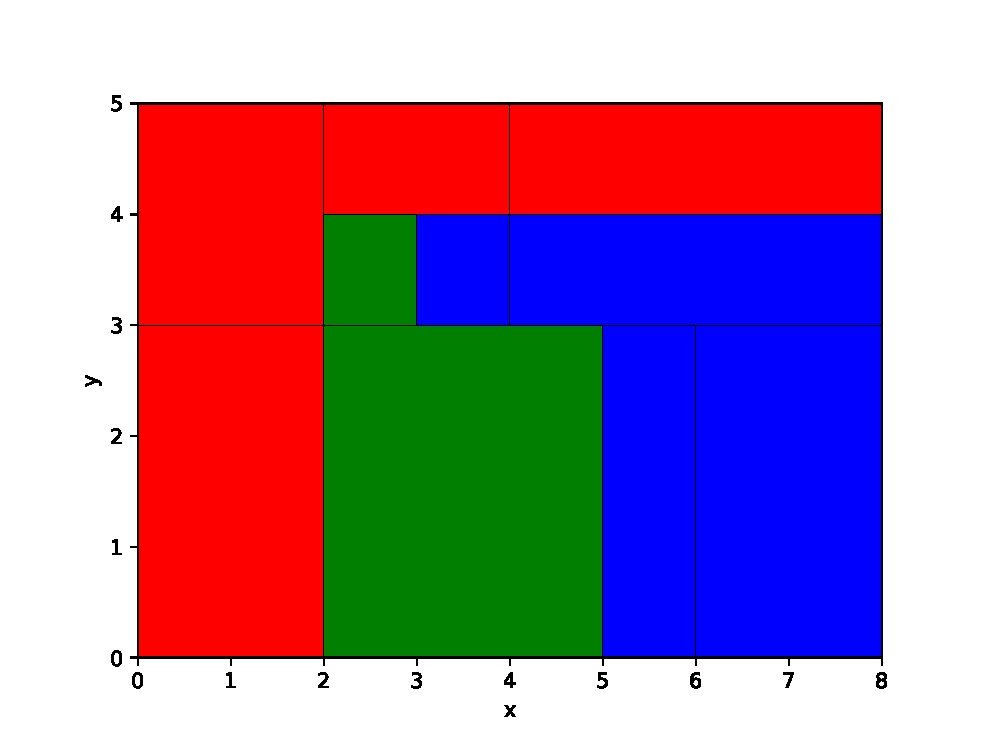
\includegraphics[width=\textwidth]{complexExample2dVisual}
        \subcaption{%
            % 2D visualization of the state space partitioning entailed by the
            % decision tree.
        }\label{fig:complexExample2dVisual}
    \end{subfigure}%

    \caption{%
        Two representations of the toy strategy introduced in
        Example~\ref{ex:runningExample}.  In~\subref{fig:complexExampleTree} the
        deterministic version of the Q-table is represented as a decision tree.
        In~\subref{fig:complexExample2dVisual} a 2D visualization of the state
        space partitioning is showed, where the colors indicate what the optimal
        action is in that area of the state space (red for $a$, green for $b$
        and blue for $c$).
    }%
    \label{fig:complexExample}
\end{figure}

The \texttt{MaxPartitions} algorithms achieves this by maximizing the size of
each partition so the strategy can be represented with a minimum number of
partitions. The basic concept of the algorithm is to try and construct as large
a partition as possible starting from a given point (typically the point
representing the minimum of each dimension) while retaining the invariant that
only one action is considered optimal in this partition. When this invariant is
violated, the new partition is stored and the operation continues from the
`corner' points of the new partition.  The pseudocode is given in
Algorithm~\ref{alg:MaxPartitions}.

\subsection{Description of the algorithm}%
\label{sub:maxPartsDescription}

The algorithm takes 4 inputs as arguments. $\mathcal{T}$ is a decision tree
representing a strategy $\sigma$ and a complete partitioning of the state space
$\mathcal{S} \in \mathbb{R}^K$; $\mathcal{C}$ is the set of constraints entailed
by $\mathcal{T}$ so that each element of $\mathcal{C}$ is a tuple $(V_i, c)$
representing the predicate $\rho(x) = x_i \le c$ of a branch node in
$\mathcal{T}$; $\mathcal{V}$ is the set of variables (dimensions); and
$p_{start}$ is the initial point the algorithm should start from.

In line 2 and 3 we define two lists. $regions$ is where we will store the
regions we identify during the algorith, and $\mathcal{P}$ is used to keep track
of points from where we will search the state space. We initialize
$\mathcal{P}$ with the single point $p_{start}$. In line 4, we start our main
loop which terminates when $\mathcal{P}$ is empty.

Line 5-11 sets up the search we are about to do from the next point in
$\mathcal{P}$. First, we initialize an empty list $exhausted$ to keep track of
the dimensions that we are done exploring. Then we sort $\mathcal{P}$ so that we
process the points in a consistent order. We then pop the first element of
$\mathcal{P}$ and uses this as $p^{\min}$ for the region we are about to create.
However, if we have already covered $p^{\min}$ in a previous iteration (by
constructing a region $\nu$ in which $p^{\min}$ is contained), we skip this
iteration and continue at line 4. Otherwise, we define $p^{\max} = p^{\min}$ so
we now have an infinitesimally small region $\nu = (p^{\min},p^{\max})$, and
finally we sort $\mathcal{C}$ in ascending order with respect to the distance to
$p^{\min}$. That is, we order $\mathcal{C}$ so that for any two consecutive
tuples $(V^m_i, c^m), (V^{m+1}_j, c^{m+1}) \in \mathcal{C}$ it holds that
$abs(c^m - p^{\min}_i) \le  abs(c^{m+1} - p^{\min}_j)$.\todo{This last part
    about sorting $\mathcal{C}$ currently isn't in the pseudocode, as it got cut
during refactoring --- but it needs to go back in!}

In line 12 we begin our search through $\mathcal{C}$ for possible candidate
bounds to grow our new region with. As mentioned, each bound is a tuple giving a
dimension $V_i$ and a constraint value $c$. We only look at the subset of
$\mathcal{C}$ where $V_i$ is not exhausted and $c > p^{\min}_i$, and we process
these bounds in sorted order according to their distance to $p^{\min}$
(currently not reflected in the pseudocode). When we find a candidate bound, we
store the current value of $p^{\max}_i$ in a variable $oldValue$ (line 14)
before updating it with the new bound (line 15).

In line 17 we do 3 different checks to see if our current region $\nu =
(p^{\min}, p^{\max})$ is now violating any requirements. First, we check if
evaluating $\nu$ in $\mathcal{T}$ only returns 1 action.  Secondly, we check if
we have moved $p^{\max}$ into an area already explored earlier (akin to the
check in line 8). And lastly, we check if the latest update to $p^{\max}_i$
moved it to the limit of the values $V_i$ can attain (denoted $V^{\max}_i$). If
neither of these are true, we continue our attempt at updating $p^{\max}$ from
line 12.

If any of the conditions are true, we proceed to check if and how we should
store the region spanned by $p^{\min}$ and $p^{\max}$. First, in line 18, we add
$V_i$ to the list of exhausted dimensions. This is because we know, that in one
way or another, expanding $p^{\max}$ in the direction of $V_i$ has violated on
of the requirements in line 17 and as such, $V_i$ should be ignored going
forward. Then in line 19, we check if $p^{\max}_i$ is still smaller than
$V^{\max}_i$. If it is, that means that we have to roll back the last update,
which we do in line 20.

\begin{algorithm}[!ht]
    \caption{Grow}\label{alg:Grow}

    \begin{algorithmic}[1]
        \Function{Grow}{$p, E, s^{\min}$}
            \State{%
                $D \gets \{
                    i \mid i \notin  E, \quad p_i < M_i, \quad i = 1,\ldots, K
                \}$ 
            }
            \State{%
                $i \gets \argmin_{i \in D}
                    \mathcal{C}_{i,p_i + 1} - \mathcal{C}_{i,p_i}$
            }

            \State{%
                $s' \gets (\mathcal{C}_{1,p_1}, \ldots,
                \mathcal{C}_{i,p_i + 1},\ldots, \mathcal{C}_{K,p_K})$
            }

            \If{%
                $|\mathcal{T}((s^{\min},s'))|$ $>$ 1 \textbf{or}
                $s'$ is explored
            }
                \State{\textbf{return} $p, E \cup {\{i\}}$}
            \ElsIf{$p_i + 1 = M_i$}
                \State{\textbf%
                    {return}
                    $(p_1, \ldots, p_i + 1, \ldots, p_K), E \cup \{i\}$
                }
            \Else%
                \State{%
                    \textbf{return} $(p_1, \ldots, p_i + 1, \ldots, p_K), E$
                }
            \EndIf%
        \EndFunction
    \end{algorithmic}

\end{algorithm}

\begin{algorithm}[!ht]
    \caption{MaxPartitions}\label{alg:MaxPartitions}

    \begin{algorithmic}[1]
        \Require{%
            $\mathcal{T}$: A binary decision tree over the domain
            $\mathbb{R}^K$ inducing the partitioning $\mathcal{A}_{\mathcal{T}}$
        }
        \Require{%
            $M$: A $K$-dimensional vector, where $M_i$ is the number of
            constraints on dimension $i$ in $\mathcal{A}_{\mathcal{T}}$
        }
        \Require{%
            $\mathcal{C}$: A $K \times M$ matrix of the constraints on each
            dimension $i$ sorted in ascending order, such that
            $\mathcal{C}_{i,j}$ is the $j$th smallest constraint in dimension
            $i$ for all $j = 1,2,\ldots,M_i$.
        }

        \State{$\mathcal{R} \gets \{\}$}
        \State{%
            $p^0 \gets (p_1, p_2, \ldots, p_K)$
            where $p_i = 0$ for all $i = 1, 2, \ldots, K$
        }
        \State{$\mathcal{P} \gets \{ p^0 \} $}

        \While{$\mathcal{P}$ is not empty}
            \State{$p^{\min} \gets \min \mathcal{P}$}
            \State{%
                $p^{\max} \gets
                (p^{\min}_1 + 1, p^{\min}_2 + 1, \ldots, p^{\min}_K + 1)
            $}
            \item

            \State{%
                $s^{\min} \gets (\mathcal{C}_{1,p^{\min}_1},
                \mathcal{C}_{2,p^{\min}_2},\ldots, \mathcal{C}_{K,p^{\min}_K})$
            }
            \State{%
                $s^{\max} \gets (\mathcal{C}_{1,p^{\max}_1},
                \mathcal{C}_{2,p^{\max}_2},\ldots, \mathcal{C}_{K,p^{\max}_K})$
            }
            \item

            \State{$\mathcal{P} \gets \mathcal{P} \setminus \{p^{\min}$\}}
            \State{$E \gets \{\}$}
            \item

            \While{$|E| < K$}

                    \State{%
                        $p^{\max}, E \gets$ \Call{Grow}{%
                            $p^{\max}, E, s^{\min}$
                        }
                    }
                \item

            \EndWhile%

            \State{%
                $s^{\max} \gets (\mathcal{C}_{1,p^{\max}_1},
                \mathcal{C}_{2,p^{\max}_2},\ldots, \mathcal{C}_{K,p^{\max}_K})$
            }
            \State{$\mathcal{R} \gets \mathcal{R} \cup \{(s^{\min},s^{\max})\}$}

            \item
            \For{$i = 1, 2, \ldots, K$}
                \If{%
                    $p^{\min}_i \neq p^{\max}_i$
                    \textbf{and} $p^{\max}_i < M_i$
                }
                    \State{$\mathcal{P} \gets \mathcal{P} \cup
                    \{(p^{\min}_1, \ldots, p^{\max}_i, \ldots,
                    p^{\min}_k)\}
                $}
                \EndIf%
            \EndFor%


        \EndWhile%

        \State{\textbf{return} $\mathcal{R}$}

    \end{algorithmic}

\end{algorithm}

Then in line 21-22, we check if there are still unexhausted dimensions, and if
so, we continue the search from line 12. Otherwise, we have have found
$p^{\max}$ that spans the largest area from $p^{\min}$ that only prescribes one
action in $\mathcal{T}$ and neither exceeds any dimensional upper limits of the
state space or expands into other found regions. We can therefore, in line 23,
add the region $\nu = (p^{\min},p^{\max})$ to the list of regions.

The last thing needed is to add new starting points to $\mathcal{P}$. This is
done in line 25-27. For every $V_i$ in $\mathcal{V}$ we create a new point $p' =
(p^{\min}_1, \ldots, p^{\max}_i, \ldots, p^{\min}_k)$ and add it to
$\mathcal{P}$ as long as long as some basic properties hold. Then we break (line
28) and continue processing the next point in $\mathcal{P}$.


\subsection{Analyzing the algorithm}%
\label{sub:maxPartsAnalysis}

In the following we provide an upper bound of the running time of
\texttt{MaxPartitions} and a proof of correctness.

For the running time, we first turn our attention to the outer while loop
iterating through $\mathcal{P}$. Since $\mathcal{P}$ is dynamically grown, we
must consider what the accumulated size during the entire run of the algorithm
can amount to. For this, we look at the case where new points are added to
$\mathcal{P}$, namely in line 27-31 where we have found a new region. We add a
point for each of the $K$ variables, barring some edge cases. This means, that
an upper bound to the number of points we must process in total is $K$ times the
number of regions we find.

The worst case number of regions the algorithm can find is on the other hand
bounded by the number of partitions (or leaf nodes) in the original tree
$\mathcal{T}$. This because either the partitioning $\mathcal{A}$ entailed by
$\mathcal{T}$ is already optimal, in which case, the algorithm will just find
one region for every leaf node in $\mathcal{T}$, or $\mathcal{A}$ is not
optimal, meaning the algorithm will find fewer (but larger) regions. Therefore,
the outer while loop is bounded by $O(KN)$ with $N$ being the number of leaf
nodes in $\mathcal{T}$.

Inside the while loop, we have two sorting operations and a for-loop. In line 6,
we sort $\mathcal{P}$, but we ignore this in our analysis, as $\mathcal{P}$ is
expected to at any time only contain a small subset of all the points entering
and exiting $\mathcal{P}$ during the algorithm. Secondly, a smart data structure
(eg.\ a heap) could sort the points at insertion and thus remove the need to
sort every time.

In line 11, however, we sort $\mathcal{C}$ according to the current $p^{\min}$.
As presented here, this sorting is unavoidable as we cannot expect to know the
correct sorting with respect to $p^{\min}$.\footnote{%
    One could imagine, that $K$ lists with the bounds in $\mathcal{C}$ sorted
    according their respective $V_i$ were stored and consulted in the following
    for-loop, thus alleviating the need to sort $\mathcal{C}$ in every
    iteration. This approach is not pursued here.
} If we assume that the sorting operation is $O(C\log C)$ with $C$ being the
size of $\mathcal{C}$, then question becomes one of estimating $C$. Also here we
have that $C$ is proportional to $N$ and $K$, as $\mathcal{C}$ is constructed
from all the predicates of the branch nodes in $\mathcal{T}$. This is at most
$N$, or rather $N-1$. Something something $\approx O(KN^2\log N)$.

\begin{theorem}
    Given a partitioning $\mathcal{A}_{\mathcal{T}}$ induced by the decision
    tree $\mathcal{T}$, the \texttt{MaxPartitions} algorithm finds the minimal
    partitioning $\mathcal{B}$ such that for any region $\nu \in \mathcal{B}$,
    $\mathcal{T}(p)$ assigns the same action $a \in Act$ to each $p \in \nu$.
\end{theorem}

\subsection{From regions to decision tree}%
\label{sub:regionsToDT}

The output of the \texttt{MaxPartitions} algorithm is a list of regions with
associated actions. For this to be of any use, we need to construct a new
decision tree to represent these state-action pairs. To this goal, we face the
issue that it is not given (and in fact, very unlikely) that the suggested
partitioning can be perfectly represented by a decision tree, as this would
require the existence of enough `clean splits' (ie.\ predicates on some variable
that perfectly divides the regions into two sets with an empty disjunction) to
arrange the entire set of regions.

Therefore, we suggest a brute-force algorithm that tries to separate the regions
as cleanly as possible. Let $\mathbf{R}$ be a list of regions $\nu \in
\mathbf{R}$ with $a_{\nu}$ being the action associated with $\nu$. We
iteratively create a branch node that splits $\mathbf{R}$ into two,
$\mathbf{R}_{low}$ and $\mathbf{R}_{high}$, based on a predicate function
$\rho(x_i,c) = x_i \le c$ with $c \in \mathbb{R}$ so that $\mathbf{R}_{low} = \{
\nu \in \mathbf{R} \mid \nu_{i,\min} \le c \}$ and $\mathbf{R_{high}} = \{ \nu
\in \mathbf{R} \mid \nu_{i,\max} > c \}$. When the list only contains a single
element $\nu$, we create a leaf node with action $a_{\nu}$ and return.

The question is how to determine $\rho(x_i,c)$, more specifically which variable
$x_i$ to predicate on and at which value $c$. Ideally, we want to split
$\mathbf{R}$ in two equally sized subsets and in a way that no single region
would have to occur in both, ie.\ we would like $\mathbf{R}_{low} \cap
\mathbf{R}_{high} = \emptyset$. For this we define an impurity measure
$I(\mathbf{R}_{low},\mathbf{R}_{high})$ that penalises the difference in size
between $\mathbf{R}_{low}$ and $\mathbf{R}_{high}$ and the size of the
disjunction between the two. Let $abs(a)$ be the absolute value of $a$ and let
$|b|$ denote the size of a set $b$, then

\[
    I(\mathbf{R}_{low}, \mathbf{R}_{high})  = abs(|\mathbf{R}_{low}| -
    |\mathbf{R}_{high}|) + |\mathbf{R}_{low} \cap \mathbf{R}_{high}|
\]


Our brute-force way of finding the predicate that minimizes $I$ is to iterate
over the dimensions in $\mathcal{S}$ and for each dimension $i$ we sort the
regions according to their upper bound. Let $\mathbf{R}_i = \{ \nu^1, \nu^2,
\ldots, \nu^n \}$ be the list sorted according to the $i$ th dimension so that
for all $\nu^j, \nu^{j+1}$ it holds that $\nu^{j}_{i,\max} \le
\nu^{j+1}_{i,\max}$. If we then let $\rho(x_i,c) = x_i \le c$ with $c =
\nu^{j}_{i,\max}$ we have $|\mathbf{R}_{low}| = j$ and |$\mathbf{R}_{high}| = n
- j$. For determining the size of $\mathbf{R}_{low} \cap \mathbf{R}_{high}$ we
simply need to count the number of regions $\nu^{j+m}$ for $m = 1, 2, \ldots,
n-j$ whose lower bound is less than our predicate bound $c$, since these regions
will appear both in $\mathbf{R}_{low}$ (because then, by definition, $\rho(x_i,c) = x_i
\le c$ will be true for $x_i = \nu^{j+m}_{i,\min}$ and $c = \nu^{j}_{i,\max}$)
and in $\mathbf{R}_{high}$ (because our sorting ensures that for all
$\nu^{j},\nu^{j+m}$ it holds that $\nu^{j}_{i,\max} \le \nu^{j+m}_{i,\max}$).

Now we can write our impurity measure in terms of these quantities:

\[
    I(\mathbf{R}_{low}, \mathbf{R}_{high}) = abs(j - (n - j)) +
    \sum^{n}_{m=1} \mathbbm{1}(\rho(\nu^{j+m}_{i,\min},\nu^{j}_{i,\max})), \quad
    \text{for all }\nu^{j} \in \mathbf{R}
\] 

where $\mathbbm{1}$ is the indicator function, $\mathbf{R}$ is the list of
regions sorted according to upper bound and $\mathbf{R}_{low}$ and
$\mathbf{R}_{high}$ are the subsets resulting from splitting on the predicate
function $\rho(x_i,c) = x_i \le c$ with $c = \nu^{j}_{i,\max}$ so that
$\mathbf{R}_{low} \subsetneq \mathbf{R}$, $\mathbf{R}_{high} \subsetneq
\mathbf{R}$ and $\mathbf{R} \subseteq \mathbf{R}_{low} \cup \mathbf{R}_{high}$.

Finding the best split, ie.\ the one that minimizes the impurity, is a $O(Kn^2)$
operation, as it requires a nested loop through all the regions for each
of the $K $dimensions (the nested loop being the final summation term over $m =
1, 2, \ldots, n - j$ for all $j = 1, 2, \ldots, n - 1$). In this work, we have
not attempted to find a faster implementation as we found that the size of
$\mathbf{R}$ obtained by using our \texttt{MaxPartitions} algorithm did not
cause performance issues.


\section{From Q-trees to Decision Tree}%
\label{sec:convergeToDT}

\subsection{Defining Q-trees}%
\label{subsec:defQTrees}

In Reinforcement Learning~\cite{Sutton1998} an agent is trying to estimate the
expected value (cost or reward) of taking and action $A$ in a state $S$. This is
called the Q-value. Let $Act$ be a finite set of actions and let $\mathcal{S}
\in \mathbb{R}^K$ be the state space (a bounded $K$-dimensional euclidean space)
then the goal is to learn the function $Q(s,a) : S, A \mapsto \mathbb{R}$ that
for any $s \in \mathcal{S}$ and $a \in Act$ maps to the Q-value of the
state-action pair.

When $\mathcal{S}$ is continuous, the $Q$-function either has to be approximated
or the state space needs to be discretized. In the latter case, $\mathcal{S}$
can be redefined in terms of well-defined bounded subspaces where each $S \in
2^{\mathbb{R}^{K}}$ now defines a smaller area of the original state space
$\mathcal{S}$ and we by $S_{i,lower}$ and $S_{i,upper}$ respectively denote the lower and
upper bound of dimension $i$ in $S$. Further, we require that $\bigcup_S S =
\mathcal{S}$.

For evaluating a particular state $s$, we say that $S = s$ iff $S_{i_{lower}}
\le s_i < S_{i_{upper}}$ for all $i = 1, \ldots, K$.  This allows for a tabular
representation of $Q(s,a)$, where the function is essentially just at
lookup-table with $|\mathcal{S}| \times |Act|$ entries. The disadvantage
of this approach is that the Q-table quickly grows very large and that many of
the discrete states are irrelevant (in the sense that they are never actually
visited). This can be remedied if close care is taken to designing the
discretization, but this would in itself impose bias onto the learning.

UPPAAL Stratego approaches the task of discretizing the state space in a
different way. Instead of schematically discretizing $\mathcal{S}$ \textit{a
priori} to the training, discretization is part of the Q-value estimation. What
happens is \ldots\todo{The introduction of a partitioning $\mathcal{A}$ and
    regions $\nu$ which I describe in Section~\ref{sec:maxParts} should probably
come here instead.}

The result is a strategy represented by a set of binary decision trees, each
pertaining to a specific action in $a \in Act$, and whose leaf nodes carries the
Q-value of taking action $a$ in the state $s$ defined by the constraints in the
branch nodes on the path from the root to the leaf. We call these trees
\textit{Q-trees} and denote by $\mathcal{T}_A$ the Q-tree for action $A \in Act$
and we define $\mathcal{T}_A(s) = Q(s,a)$ when $A=a$. Given the complete set of Q-trees
the matter of choosing the optimal action in a state $s$ can --- for a greedy
policy $\pi$ and with the Q-values representing expected cost --- be defined as
$\pi(s) = \argmin_{a\in Act} \mathcal{T}_A(s)$.


\subsection{Converting to decision tree}%
\label{subsec:convertQTtoDT}

With Definition~\ref{def:qTree} we can now consider how to construct a single
decision tree $\mathcal{T}$ so that $\pi(s) = \argmin_{a \in Act}
\mathcal{T}_A(s) = \mathcal{T}(s)$ for all $s \in \mathcal{S}$. That is, instead
of a Q-tree we will construct a decision tree where the leaf nodes carries the
action $A$ that satisfies $A = \argmin_{a \in Act} T_A(\lambda(l))$ for
a given leaf $l$. In the following, we will present the procedure for doing so
in general terms while the full specification of the algorithm is available in
Appendix~\ref{app:qTreeConversion}.

First, let $\mathcal{L}$ be the set of every leaf in the set of Q-trees and let
each leaf $l \in \mathcal{L}$ be defined as $l = (S^{l}, a_l, q_l)$ where $S^{l} =
\lambda(l)$ in $T_A$, $a_l$ is the action of the Q-tree $l$ originally belonged to
and $q_l$ is the Q-value of taking action $a_l$ in state $S^{l }$ (we use
superscripts in $S^l$ to avoid notational clutter when we later need to index
variables and bounds in $S^{l_i}$ and $S^{l_j}$ at the same time). We sort
$\mathcal{L}$ in ascending order according to $q_l$ (meaning $l_0$ has the best
Q-value of any leaf) and use the first leaf, $l_0$, to build the first path in
the tree. This path requires $2 \times K$ branch nodes, one for each lower and
upper bound of each dimension in  $S^{l}$.

The decision about the order in which to predicate the branch nodes on each
variable bound can and will greatly affect the size of the tree. However, as
determining the optimal ordering of predicates is computationally
infeasible~\cite{HYAFIL197615}, we will simply resort to a randomized picking
order.  For the root node $v_0$, we thus pick a variable $i$ and a bound $j$ at
random and set $\rho(v_0) = x_i \le c$ where $c = S^{l_0}_{i,j}$. If $j$ is a
lower bound, then we set the left child node to a dummy leaf (we will complete
this subtree later) and construct a new branch node for the right child from the
remaining pairs of $i, j$ in $S^{l_0}$ and vice-versa if $j$ is an upper bound.
We continue this procedure until $S^{l_0} = \lambda(l_0)$ holds true in the tree
under construction.

For inserting the another leaf, $l_j$, we now need to check at each branch node
$v_m$ whether we should insert in the left subtree, in the right subtree or in
both.  In other words, we do two checks: if $\rho(v_m)$ is $true$ for $x_i =
S^{l_j}_{i,lower}$ we continue the insertion procedure in the left subtree.  If
$\rho(v_m)$ is $false$ for $x_i = S^{l_j}_{i, upper}$ we \textit{also} insert
$l_j$ into the right subtree. If both cases evaluates to $false$, we
\textit{only} do the insertion in the right subtree. If we encounter a dummy
leaf, we either construct a new branch node as we did for the initial path, ie.\ by
randomly picking a still unchecked variable and bound to use for the predicate
function, or --- in the case that $S^{l_j} = \lambda(l_j)$ already holds true
for the tree under construction --- simply insert $l_j$ instead of the dummy.

If we encounter a non-dummy leaf we can exploit the fact that the leaf nodes are
inserted in a sorted order according to their Q-values. This ensures that if we
encounter $l_i$ during insertion of $l_j$ then we know that $q_i \le  q_j$ and
we can therefore safely stop the insertion of $l_j$ (in this particular subtree)
as we know that for all $s \in S^{l_i} \cap S^{l_j}$ it must hold true that
$\pi(s) = a_i$.

When all leaf nodes from the set of Q-trees have been processed the resulting
tree $\mathcal{T}$ represents the exact same strategy but now without any notion
of Q-values. In the Python library built for this paper, it is possible to
export a decision tree representation to a Q-tree representation that can then
be imported into \texttt{UPPAAL Stratego} in order to test the performance of
the strategy. This is done by for each $A \in Act$ creating
$\mathcal{T}_A$ as a copy of $\mathcal{T}$ and then for every leaf $l$ setting
$q_l = 0$ if $a_l = A$ and $q_l = 999$ if $a_l \neq A$.

\section{Minimization techniques}%
\label{sec:minimization}

As we can give no guarantees to the minimality of the decision tree created from
a set of Q-trees, $\mathcal{T}$ can grow very large and even contain more paths
than all the Q-trees combined. This is unwanted, and we therefore present
several minimization techniques that can drastically decrease the size of
$\mathcal{T}$.

\subsection{Simple pruning}%
\label{sub:simplePrune}\todo{This subsection and the next
    (Section~\ref{sub:simplePrune} and~\ref{sub:anaPrune}) I am not at all
    certain about how to actually approach yet. The simple pruning is so simple,
    that it is almost redundant to describe and the analytical pruning is only
partially implemented and not very systematic yet.}


The algorithm described in Section~\ref{subsec:convertQTtoDT} naively inserts
leaf nodes without any consideration of optimality (except what little is given
from the fact that leaf nodes are inserted in order of Q-value). This yields
some obvious cases where branch nodes can be pruned away.

Say we have a path $p = \{v_0, v_1, \dots, v_n \}$ where both children of $v_n$ 
are leaf nodes, $l_i$ and $l_j$. If $a_i = a_j$ then the predicate at $v_n$
bears no significance and we can replace that node with either $l_i$ or $l_j$.
Now the child of $v_{n-1}$ that used to be $v_n$ is a leaf, which might again
result in a situation where $v_{n-1}$ has two leaf children with the same
action. Thus, we iteratively check for this condition all the way up through the
tree, pruning any such cases.

Something something $\lambda(v_n) = \lambda(l_i) \cup \lambda(l_j) \land a_i =
a_j \implies \pi(\lambda(v_n)) = a_i = a_j$.

\subsection{Analytical pruning}%
\label{sub:anaPrune}

\lipsum[1]


\subsection{Empirical pruning}%
\label{sub:empPrune}

During training, the partitioning scheme used by UPPAAL Stratego to discretize
the state space is explorative in the sense that it is non-deterministic when it
creates new partitions. As it goes along, the algorithm discovers areas of
interest where the choice of action seem to have greater impact on the overall
cost and it then refines its partitioning in these areas.

This leads to somewhat abundance of partitions early on in the training, where
more or less random splits turns out to not influence the decision making. These
splits are carried on into the final strategy and they are also imported into
our converted decision tree where the merging of the different Q-trees actually
amplify this abundance.

This has two consequences. One is that the state space will be partitioned in
such a way that neighboring partitions actually prescribe the same action, but
do not necessarily appear as neighboring leafs in the strategy tree (ie.\ they
do not have the same parent). We will deal with this problem in the
Section~\ref{sec:maxParts}. The other consequence is that we end up with a lot
of leaf nodes that in practice will never be visited, as the system that is
modeled either never end up in such a state or because the strategy has the
controller behave in such a way, that such a state is always avoided.\todo{This
    entire intro should possible be moved to the beginning of this section
    (Section~\ref{sec:minimization}). Also, I would like to be able to describe
    the `issue' stemming from UPPAAL more precisely but for that, I probably
need help from Peter.}

To deal with this, we employ a technique we call \textit{empirical pruning}. In
contrast to our other effort, this technique is not based on any analysis of the
tree structure or state space but instead employs sample data to prune the tree
of any leaf nodes that are either never or rarely visited. This have the
drawback, that we loose our ability to give guarantees about the strategy, as our
sampling \textit{might} just miss an important edge case that our empirically
pruned strategy then does not know how to handle. On the other hand, given a
large a enough sample, this risk is negligible since such a case would most
likely have been just as rare during training, meaning the strategy would not
even be ready to deal with it properly had it not been pruned from the tree.

The way it works is by gathering a sample of data points $D = \{ s_0, s_1,
\ldots, s_T\}$ representing the state of the system at each time step during a
run (or preferably several runs) where the controller acts according to a well
trained strategy represented by the tree $\mathcal{T}$. For each state $s_t \in
D$ we increase a counter at the leaf node at the end of the path that came from
evaluating $\mathcal{T}(s_t)$.

When this process is done with a sufficiently large $D$, we can prune all the
leaf nodes that were never visited or rarely visited. If we prune the never
visited nodes, we call it \textit{zero-pruning}. Pruning nodes visited once is
called \textit{one-pruning} and so forth. The pruning is simply done by removing
every branch node with a leaf child that is never visited and instead
`promoting' the subtree that is its other child.

For example, if we have a path $p = \{ \ldots, v_{i-1}, v_i, v_{i+1}, \ldots \}$
and $v_i$ has a leaf node $l$ for its other child and we see from sampling that
$l$ is never visited, then the constraint that $v_i$ represent has no relevance
for $v_{i+1}$. Therefore, we remove $v_i$ and set $v_{i+1}$ as a child of
$v_{i-1}$ instead. Doing this iteratively from the `left-most' leaf and all the
way through the tree can lead to substantial reductions, as we will show in
Section~\ref{sec:experiments}, and provided that the sample size is large enough
the performance of the pruned strategy stays on par with the original.

